\documentclass[11pt]{article}
\usepackage[utf8]{inputenc}
\usepackage[T1]{fontenc}
\usepackage[margin=0.85in]{geometry}
\usepackage{amsmath,amssymb,amsthm}
\usepackage{booktabs}
\usepackage{array}
\usepackage{url}
\usepackage{microtype}
\usepackage{graphicx}
\usepackage{caption}
\usepackage{xcolor}
\usepackage{listings}
\usepackage[hidelinks]{hyperref}
\makeatletter\g@addto@macro{\UrlBreaks}{\do\_\do\.\do\/}\makeatother
\emergencystretch=3em
\tolerance=2000
\renewcommand{\topfraction}{0.9}\renewcommand{\textfraction}{0.07}\renewcommand{\floatpagefraction}{0.85}
% generated by gen_inputs.py; do not edit
\newcommand{\LeanSha}{fac6c85f9e6c0bd7b60861a9e1286a56283ef211d006630351ebb3c0e9e39454}
\newcommand{\LeanShaShort}{fac6c85f9e6c}
\newcommand{\CtlSha}{0beb41c999802886a4ee02d29875a01a064da2ea8936fc3b577dbe707db92ed5}
\newcommand{\CtlShaShort}{0beb41c99980}
\newcommand{\OwnerSha}{a28ce47e70c64ce9edb0496cba41a698cb40a93fc622927025f801501e740d04}
\newcommand{\OwnerShaShort}{a28ce47e70c6}
\newcommand{\NDecl}{26}
\newcommand{\ProdSec}{1004.9}
\newcommand{\ReSec}{12.1}
\newcommand{\ReCtlSec}{9.1}
\newcommand{\GPhase}{4.09\times10^{-5}}
\newcommand{\GDensity}{4.06\times10^{-5}}
\newcommand{\GAmp}{1.64\times10^{-4}}
\newcommand{\GZero}{7.79\times10^{-13}}
\newcommand{\GZeroDist}{0.3355}
\newcommand{\GBound}{-1.381\times10^{-3}}
\newcommand{\GNearOne}{1.381\times10^{-3}}
\newcommand{\GNearOneExact}{1.3809\times10^{-3}}
\newcommand{\GNearOneDiff}{6.9\times10^{-8}}
\newcommand{\GRefAmp}{0.2497}
\newcommand{\GRefOrder}{1.013}
\newcommand{\GOrder}{2.000}
\newcommand{\GIso}{1.78\times10^{-7}}
\newcommand{\GGs}{4.31\times10^{-14}}
\newcommand{\NGates}{14}
\newcommand{\NGatesPass}{14}
\newcommand{\RefEpsB}{1.23\times10^{-2}}
\newcommand{\TangFine}{-3.56\times10^{-9}}
\newcommand{\RefAmpFirst}{2.65\times10^{-2}}
\newcommand{\RefAmpLast}{1.63\times10^{-3}}
\newcommand{\StrOneFirst}{1.27\times10^{-6}}
\newcommand{\StrOneLast}{3.56\times10^{-9}}
\newcommand{\NSweep}{25}
\newcommand{\Grid}{32}
\newcommand{\Periods}{6}
\newcommand{\SPP}{200}
\newcommand{\Eps}{1\times10^{-3}}
\newcommand{\CxOmegaMax}{1.6\times10^{-12}}
\newcommand{\CxOmegaMin}{1.9\times10^{-14}}
\newcommand{\CxAmpMax}{2.4\times10^{-9}}
\newcommand{\HeKs}{3.0038}
\newcommand{\HeHbarTwoM}{0.52218}
\newcommand{\HeThrQR}{0.5662}
\newcommand{\HeThrLo}{0.56609}
\newcommand{\HeThrHi}{0.56633}
\newcommand{\HeSilentHi}{0.90}
\newcommand{\HeFirstUnd}{0.95}
\newcommand{\HeNSilent}{18}
\newcommand{\HeNUnd}{54}
\newcommand{\HeNRows}{72}
\newcommand{\HeSupRoton}{2.66}
\newcommand{\HeThrRotonTab}{0.5697}
\newcommand{\HeRotonK}{1.95}
\newcommand{\HeNoErrK}{0.05, 0.10}
\newcommand{\HeNoErrMargins}{0.0166 vs 0.0912; 0.0329 vs 0.1290}
\newcommand{\HeEpsRatio}{0.205}
\newcommand{\HeEpsRatioMin}{0.176}
\newcommand{\HeMarginS}{0.1665}
\newcommand{\HeMarginT}{0.2885}
\newcommand{\HePhonRel}{0.35}
\newcommand{\HFQueries}{30}
\newcommand{\HFId}{popoff4rtem/\allowbreak{}2D-\allowbreak{}Neutron-\allowbreak{}Diffraction-\allowbreak{}Dataset-\allowbreak{}for-\allowbreak{}Discriminative-\allowbreak{}Models}
\newcommand{\HFSha}{648119c2030c5352c37a305deb74aa8ec84a4402}
\newcommand{\HFBig}{4.38}

\lstset{basicstyle=\ttfamily\scriptsize,aboveskip=4pt,belowskip=4pt,columns=fullflexible,keepspaces=true,breaklines=true,
  frame=single,framesep=3pt,xleftmargin=4pt,xrightmargin=4pt,upquote=true,
  keywordstyle=\bfseries,morekeywords={theorem,lemma,def,noncomputable,import,namespace,open,end,axiom,by,sorry},
  escapeinside={(*@}{@*)}}
\newtheorem{theorem}{Theorem}
\newtheorem{lemma}[theorem]{Lemma}
\theoremstyle{remark}
\newtheorem{remark}[theorem]{Remark}
\newcommand{\tier}[1]{\textsf{[#1]}}
\newcommand{\lean}[1]{\texttt{#1}}
\newcommand{\ks}{k_s}
\newcommand{\SB}{S_{\mathrm B}}
\newcommand{\eB}{\varepsilon_{\mathrm B}}

\title{The Bogoliubov structure factor under the dual-scale envelope $\sqrt{k/2k_s}$:\\
kernel-checked shape theorems, a one-sided diffraction test,\\
and a Gross--Pitaevskii linear-response check in rusty-SUNDIALS}
\author{Xavier Callens (SocrateAI Lab)}
\date{Preprint v1, 2026-10-25}
\hypersetup{pdftitle={The Bogoliubov structure factor under the dual-scale envelope: kernel-checked shape theorems,
a one-sided diffraction test, and a Gross-Pitaevskii linear-response check}, pdfauthor={Xavier Callens}}

\begin{document}
\maketitle
\begin{center}\small doi:10.5281/zenodo.23646117 \quad (not peer reviewed)\end{center}


\noindent\textbf{AI-assistance disclosure.} This preprint, its Lean code, its Rust and Python code and its claim ledger
were produced by AI agents (Claude, Anthropic) under the author's direction. The author is responsible for the content.
No human has audited the Lean statements for adequacy, and no human referee has checked the hand proofs.

\begin{abstract}
For the zero-temperature weakly interacting Bose gas, the Bogoliubov static structure factor is
$\SB(k)=\varepsilon_0(k)/\eB(k)$, where $\varepsilon_0=\hbar^2k^2/2m$ and $\eB=\sqrt{\varepsilon_0(\varepsilon_0+2gn)}$.
With $\ks=2mc/\hbar$ it equals $k/\sqrt{\ks^2+k^2}$.

\textbf{Tier A} (kernel-checked, Lean v4.34.0-rc2 in the QuantumFluids project environment; axioms within
\{\lean{propext}, \lean{Classical.choice}, \lean{Quot.sound}\}; planted \lean{sorry} and planted-axiom controls caught).
We prove \NDecl{} statements about these model formulas:
\begin{itemize}
\item the envelope $\SB\le\sqrt{k/2\ks}$, with equality exactly at $k=\ks$;
\item strict monotonicity of $\SB$;
\item the two-sided phonon bound $k/(\ks+k)<\SB<k/\ks$;
\item $\SB<1$, the rate $1-\SB\le\ks^2/k^2$ and the limit $\SB\to1$;
\item a \emph{diffraction test}: a structure factor that rises above the envelope is not $\SB$; and, \emph{given}
Feynman's inequality as a hypothesis, the measured dispersion is then not Bogoliubov.
\end{itemize}
The test's controls are kernel-checked too: it fires on the free value $S=1$ and never fires on $\SB$.

\textbf{Tier X} (floating point; supports no claim). A new linear-response module in the rusty-SUNDIALS crate
\texttt{qf-gpe2d} recovers $\eB(k)$ from Gross--Pitaevskii dynamics to $\GPhase$ relative error. All \NGates{}
numeric gates pass, including $g=0$ and splitting negative controls. Along the way we found that the pinned upstream
reference data are reproduced by a reused-phase composition, not by the symmetric Strang step; the upstream source
itself was not inspected. The crate's own \texttt{step}/\texttt{evolve} use the same composition. In linear response that
composition converges only at first order in the amplitude; a new true Strang option converges at second order.

\textbf{Real data} (Tier L inputs, Tier X evaluation). Using the published $^4$He dispersion table, the threshold at the
roton is $\sqrt{Q_R/2\ks}=\HeThrQR$. Assuming Feynman's inequality, the dispersion table alone says the test is silent
for $k\le\HeSilentHi$\,\AA$^{-1}$ and cannot decide from $\HeFirstUnd$\,\AA$^{-1}$ upward, including the roton.

\textbf{Unmet deliverable: HuggingFace.} The task asked for a HuggingFace dataset to illustrate the result. That was not delivered:
a search of \HFQueries{} HuggingFace queries found no structure-factor dataset, so no HuggingFace data illustrate this
paper. The published $^4$He table, which is not on HuggingFace, is the real-data illustration instead.

There is no novelty in mathematics or physics: the core inequality is $(k-\ks)^2\ge0$. What is offered is a
kernel-checked statement in the owner project's vocabulary, a tested solver extension, and honest bookkeeping.
\end{abstract}

\paragraph{Tiers.} \tier{A}: a Lean statement checked by the kernel, axioms within the allowlist, planted controls
caught. A Tier~A tag attaches to the Lean statement about the \emph{model formulas}, never to its physical gloss.
\tier{L}: a cited source, quoted verbatim in the ledger with line numbers of the alphaXiv text extraction. Here L
covers verbatim \emph{data values and quotes}. That is looser than the Elenchus L tier, which accepts theorem
statements only: Elenchus \texttt{citation\_check.py} refuses BS-L-0001 under its honest kind \texttt{data\_value}
(\texttt{CITE\_KIND}). With the kind forced to \texttt{theorem}, used only to test whether the quotes are verbatim, it
accepts BS-L-0001 and BS-L-0004; that probe is not a Tier~L verdict. The BS-L-0004 source file is an excerpt written by
the producing agent, not the full extraction. All three cited papers were checked against fresh alphaXiv reads by an
independent agent.
\tier{C}: an argument or human proof that is not machine-checked. \tier{X}: floating-point exploration, which never
supports a claim. Identifiers such as \texttt{BS-A-0001} refer to \texttt{ledger/ledger.json}
(Section~\ref{sec:ledger}).

\paragraph{Dependencies.} Nothing here depends on the openai/math release or on any triangular-lattice theorem. The
conditionalities are different, and they are stated where they enter:
\begin{enumerate}
\item the zero-temperature Bogoliubov model formulas, taken as \emph{definitions} in Lean;
\item Feynman's inequality $\varepsilon(k)\le\varepsilon_0(k)/S(k)$, which enters only as the explicit hypothesis
\lean{hfeyn} of \lean{diffraction\_test\_dispersion};
\item the measured sound speed $c$, which sets $\ks$ whenever the test is applied to data.
\end{enumerate}

\section{System, units and regime}\label{sec:physics}
Consider a uniform three-dimensional Bose gas of density $n$ and mass $m$ with contact coupling $g$, at $T=0$, in the
weak-coupling (Bogoliubov) regime $na^3\ll1$. The sound speed is $c=\sqrt{gn/m}$ and the healing length is
$\xi=\hbar/(\sqrt2\,mc)$. We write
\[
\ks:=\frac{2mc}{\hbar}=\frac{\sqrt2}{\xi},\qquad \hbar c=:h_c .
\]
Then $\varepsilon_0(k)=\hbar^2k^2/2m=h_c k^2/\ks$ and $2gn\,\varepsilon_0=(h_c k)^2$, so the Bogoliubov dispersion is
\begin{equation}\label{eq:eB}
\eB(k)^2=\varepsilon_0(\varepsilon_0+2gn)=(h_ck)^2+(h_ck^2/\ks)^2 .
\end{equation}
This is exactly the owner project's \lean{bogoliubovSq hc ks k} (Listing~\ref{lst:owner}) \tier{C, BS-C-0002}.
The Bogoliubov static structure factor is $\SB=(u_k-v_k)^2=\varepsilon_0/\eB$ \tier{C, BS-C-0002}. In Lean it is a
\emph{definition}, so the Bijl--Feynman relation $\eB=\varepsilon_0/\SB$ holds by construction.

The quantity $\sqrt{k/2\ks}$ comes from the owner's ``dual-scale'' reading of the dispersion. Write
$\ell(k)=\varepsilon(k)^2/(h_c^2k^3)$. Bogoliubov gives $\ell=1/k+k/\ks^2\ge2/\ks$ (\lean{ell\_ge}). For a Feynman
spectrum $\varepsilon_0/S$ the same bound is equivalent to $S^2\le k/2\ks$ (\lean{feynman\_ge\_iff}). The owner
project proves both. It does not name $\SB$, and it does not state $\SB\le\sqrt{k/2\ks}$.

\paragraph{What the theorems say and do not say.} They are statements about the formulas above. They say nothing
about any real fluid unless the formulas describe it. Applied to data they become a \emph{one-sided} test: a measured
$S(k)$ above $\sqrt{k/2\ks}$ at some $k$ is incompatible with the Bogoliubov $\SB$ of the same $\ks$. A measured $S$
below the envelope proves nothing.

\section{Step-by-step human demonstration}\label{sec:human}
This section is written for a strong undergraduate. Every step is proved by hand and then paired with the Lean
declaration that checks it \tier{A, BS-A-0001 to BS-A-0008}. Throughout, $h_c>0$, $k>0$ and $\ks>0$, and
$x:=k/\ks$.

\paragraph{Step 1: the dispersion in project variables.} By \eqref{eq:eB},
$\eB^2=\varepsilon_0^2+(h_ck)^2>0$ because $h_ck>0$. Lean: \lean{bogoliubovSq\_pos}, \lean{epsBog\_sq}.

\paragraph{Step 2: closed form.} $\SB^2=\varepsilon_0^2/\eB^2$. Divide numerator and denominator by $h_c^2k^2/\ks^2$:
\[
\SB^2=\frac{h_c^2k^4/\ks^2}{h_c^2k^2+h_c^2k^4/\ks^2}=\frac{k^2}{\ks^2+k^2}.
\]
$h_c$ drops out. Since $\SB>0$ (a quotient of positive numbers), $\SB=k/\sqrt{\ks^2+k^2}$. Lean: \lean{sBog\_pos},
\lean{sBog\_sq}, \lean{sBog\_eq\_closed}.

\paragraph{Step 3: the envelope.} Both sides are positive, so
$\SB^2\le k/(2\ks)\iff 2\ks k^2\le k(\ks^2+k^2)\iff 0\le k(k-\ks)^2$.
The last inequality is true. Taking square roots, which preserve order on $[0,\infty)$, gives
$\SB\le\sqrt{k/2\ks}$. Lean: \lean{sBog\_sq\_le}, \lean{sBog\_le\_sqrt}.

\paragraph{Step 4: sharpness.} Equality in Step~3 holds iff $k(k-\ks)^2=0$. Since $k>0$, that means $k=\ks$,
the self-dual wavenumber. Lean: \lean{sBog\_sq\_eq\_iff}. The hypotheses can be met, and the equality case occurs:
$\SB(1)^2=1/2$ for $h_c=\ks=1$ (\lean{nonvacuous\_selfdual}).

\paragraph{Step 5: the second route through the owner's lemmas.} The Feynman energy built from $\SB$ is
$\varepsilon_0/\SB=\eB$ (by construction, \lean{feynman\_sBog\_exact}). So
$\ell=1/k+k/\ks^2\ge 2/\ks$, since $1/k+k/\ks^2-2/\ks=(k-\ks)^2/(k\ks^2)$. By \lean{feynman\_ge\_iff} this is
again $\SB^2\le k/2\ks$. Lean: \lean{sBog\_sq\_le\_via\_project}. This route checks that the new statement agrees with
the project's existing vocabulary. It is not independent evidence.

\paragraph{Step 6: monotonicity.} $\SB^2=1-\ks^2/(\ks^2+k^2)$ is strictly increasing in $k$. Positive numbers
with increasing squares are increasing. Lean: \lean{sBog\_sq\_lt\_sq}, \lean{sBog\_strictMonoOn}.

\paragraph{Step 7: phonon regime.} $\ks<\sqrt{\ks^2+k^2}<\ks+k$, where the right inequality is
$\ks^2+k^2<\ks^2+2\ks k+k^2$. Dividing $k$ by these gives
\[
\frac{k}{\ks+k}<\SB<\frac{k}{\ks}=\frac{\hbar k}{2mc}.
\]
So $\SB\sim\hbar k/2mc$ as $k\to0$, with relative error below $k/\ks$. Lean: \lean{phonon\_lower\_lt\_sBog},
\lean{sBog\_lt\_phonon}.

\paragraph{Step 8: approach to the free particle.} $\SB<1$ because $k<\sqrt{\ks^2+k^2}$. Since $0<\SB<1$,
$1-\SB\le(1-\SB)(1+\SB)=1-\SB^2=\ks^2/(\ks^2+k^2)\le\ks^2/k^2$. The bound tends to 0, so $\SB\to1$ as $k\to\infty$.
Lean: \lean{sBog\_lt\_one}, \lean{one\_sub\_sBog\_le}, \lean{sBog\_tendsto\_one}, and \lean{epsBog\_eq\_epsFree\_div\_sBog}
for $\eB=\varepsilon_0/\SB$.

\paragraph{Step 9: the diffraction test, model level.} Step~3 contraposed: if $S>\sqrt{k/2\ks}$ then $S\ne\SB(k)$.
Lean: \lean{diffraction\_test\_model}. For $S>0$, $\sqrt{k/2\ks}<S\iff k/2\ks<S^2$ (\lean{peak\_sqrt\_iff\_sq}).

\paragraph{Step 10: Feynman's inequality (not formalized).} \tier{C, BS-C-0001.} At $T=0$, let $S(k,\omega)\ge0$ be the
dynamic structure factor per particle. Its zeroth moment is $\int S(k,\omega)\,d\omega=S(k)$, and the f-sum rule gives
$\int\hbar\omega\,S(k,\omega)\,d\omega=\varepsilon_0(k)$. If $\varepsilon(k)$ is the lowest energy of a state reached
from the ground state by the density operator $\rho_k$, then $S(k,\omega)$ vanishes for $\hbar\omega<\varepsilon(k)$, so
\[
\varepsilon(k)\,S(k)\le\int\hbar\omega\,S(k,\omega)\,d\omega=\varepsilon_0(k),\qquad\text{i.e.}\qquad
\varepsilon(k)\le\varepsilon_0(k)/S(k).
\]
This is the inequality usually attributed to Feynman~\cite{feynman}. It is used here only as a stated hypothesis.
Identifying the measured single-excitation branch with the lowest density-channel energy is a further assumption
(Section~\ref{sec:helium}).

\paragraph{Step 11: the diffraction test, dispersion level.} Assume $\varepsilon^2\le(\varepsilon_0/S)^2$
(the hypothesis \lean{hfeyn}) and $S^2>k/2\ks$. Then
\[
\varepsilon^2\le\frac{\varepsilon_0^2}{S^2}<\varepsilon_0^2\cdot\frac{2\ks}{k}=\frac{2h_c^2k^3}{\ks}
\le h_c^2k^2\Bigl(1+\frac{k^2}{\ks^2}\Bigr)=\eB^2 ,
\]
where the last step is $2x\le1+x^2$. So $\varepsilon^2\ne\eB^2$: the dispersion is not Bogoliubov.
Lean: \lean{diffraction\_test\_dispersion}, which reduces to the owner's \lean{not\_bogoliubov\_of\_structure\_factor}.

\paragraph{Step 12: controls of the test.} \emph{Positive:} the free value $S=1$ makes the test fire at $k=\ks$,
since $\sqrt{1/2}<1$. More generally $\sqrt{k/2\ks}<1$ for $k<2\ks$, and $k/\ks<1$ for $k<\ks$, which breaks the
phonon bound. Lean: \lean{diffraction\_fires\_free\_at\_selfdual}, \lean{free\_S\_one\_violates},
\lean{free\_S\_one\_violates\_phonon}. \emph{Negative:} the test never fires on $\SB$ itself, by Step~3. Lean:
\lean{diffraction\_silent\_on\_sBog}. A caveat from the round-1 verifier: $S=1$ is the $c\to0$ limit, where $\ks\to0$
too. The control fixes $\ks$, so it is a weak control.

\section{The Lean formalization}\label{sec:lean}
\paragraph{Files and toolchain.} The claimed module is
\path{results/autoresearch/2026-10-25/H8/contribution/Autoresearch_SkBoundShape.lean} (sha256 \LeanShaShort\ldots), in
namespace \lean{QuantumFluids.AutoresearchSkBoundShape}. Planted controls live only in
\path{Autoresearch_SkBoundShapeControls.lean} (sha256 \CtlShaShort\ldots). The module imports the owner's compiled
\lean{DualLength} from SocrateAI-Scientific-QuantumFluids at commit
\texttt{10f74daf1b39d2ac51a785452329fff0003cfc83} (\path{lean_src/DualLength.lean}, sha256 \OwnerShaShort\ldots). The
toolchain is Lean v4.34.0-rc2 with Mathlib \texttt{85e3a25e006c35636f0e53b0e9296caca2685bc0} (qf-lake), invoked
directly as \texttt{lean} with \texttt{LEAN\_PATH} set to the qf-lake build and package libraries. The file does not
import Mathlib itself.

\paragraph{Gate record.}
\begin{itemize}
\item Producer compile (Stage~1): rc~0 in \ProdSec\,s, no warnings or errors, \NDecl{} \lean{\#print axioms} lines, all
within the allowlist. Earlier attempts timed out on disk~I/O starvation, and one failed with two proof errors that
were then fixed; all are kept in \path{contribution/attempt*.json}.
\item Paper-stage recompile, by a separate agent instance using the producer's runner on the unchanged file (same
sha256): main rc~0 in \ReSec\,s, \NDecl{} lines, nothing outside the allowlist; controls rc~0 in \ReCtlSec\,s, both
controls flagged. This is a kernel re-check by another AI agent instance. It is \emph{not} a human audit and not a
statement-adequacy review.
\item The claimed file contains no \lean{sorry}, \lean{admit}, \lean{native\_decide} or \lean{axiom} declaration
(asserted by \texttt{gen\_inputs.py}).
\item The round-1 file \path{H8/Autoresearch_SkBound.lean} was recompiled by an independent verifier agent with
verdict ACCEPT\_WITH\_CORRECTIONS. Its KEEP was obtained on a third, infrastructure retry outside the preregistered
two-attempt rule, and is labelled that way.
\end{itemize}
The controls file exits rc~0 even though it contains a \lean{sorry} and a planted axiom. That is why the axiom
audit, not the exit code, is the gate.

\lstinputlisting[caption={Owner definitions and lemmas used (QuantumFluids \texttt{DualLength.lean}; proofs elided).},label=lst:owner]{gen/owner.lst}
\lstinputlisting[caption={Definitions in the claimed module (verbatim).},label=lst:defs]{gen/defs.lst}
\lstinputlisting[caption={Round-1 theorems, re-proved under the same names (statements verbatim, proofs elided).},label=lst:r1]{gen/round1.lst}
\lstinputlisting[caption={Shape theorems (statements verbatim, proofs elided).},label=lst:shape]{gen/shape.lst}
\lstinputlisting[caption={The diffraction test and its in-file controls (statements verbatim, proofs elided).},label=lst:test]{gen/test.lst}
\lstinputlisting[caption={Planted controls file, in full. These are not claims.},label=lst:ctl]{gen/controls.lst}

\paragraph{Axiom audit, paper-stage recompile (verbatim; Lean's line-wrap continuations joined).}
\lstinputlisting[basicstyle=\ttfamily\scriptsize]{gen/axioms_re.txt}
\paragraph{Planted controls, paper-stage recompile (same convention).}
\lstinputlisting[basicstyle=\ttfamily\scriptsize]{gen/axioms_rectl.txt}
\texttt{gen\_inputs.py} extracts every listing from the source files, byte for byte, into \texttt{gen/*.lean}. The
typeset \texttt{gen/*.lst} copies differ only in that non-ASCII symbols are escaped to LaTeX glyphs.

\section{Numerics in rusty-SUNDIALS}\label{sec:numerics}
All numbers in this section are \tier{X}: floating-point, producer-checked only, supporting no claim.

\paragraph{Method.} The crate \texttt{qf-gpe2d} integrates the 2D Gross--Pitaevskii equation
$i\psi_t=-\tfrac12\nabla^2\psi+g|\psi|^2\psi-\mu\psi$ by Fourier split-step on a periodic grid, with $\hbar=m=1$,
$n_0=g=1$, so $c=1$, $\ks=2$ and $\xi=1/\sqrt2$. The new module \texttt{linear\_response}:
\begin{enumerate}
\item relaxes the uniform ground state in imaginary time from a perturbed start (max $||\psi|^2-n_0|=\GGs$);
\item applies a weak phase kick $\psi\to\psi\,e^{i\epsilon\cos k\cdot r}$ or density kick
$\psi\to\psi\sqrt{1+\epsilon\cos k\cdot r}$ on one grid wavevector;
\item records the density cosine component $A(t)$ and reads $\omega$ from zero-crossing times and from a
least-squares sinusoid fit.
\end{enumerate}
Linearizing the GP equation gives $\omega^2=\varepsilon_0(\varepsilon_0+2gn)$. After a phase kick, continuity gives
$A(t)=(nk^2\epsilon/\omega)\sin\omega t$, so the amplitude yields a second estimate $S_\mathrm{amp}=A_\mathrm{max}/(2n
\epsilon)=\varepsilon_0/\omega$ \tier{C, BS-C-0003}. A classical GP field has no quantum density fluctuations, so
$S=\varepsilon_0/\omega$ is the Bijl--Feynman identification, not an independent measurement of a quantum $S(k)$.
This is the same by-construction point as \lean{feynman\_sBog\_exact}.

The sweep uses a $\Grid\times\Grid$ grid, \NSweep{} wavevectors with $k/\ks$ from 0.05 to 5, \Periods{} periods,
\SPP{} steps per period and $\epsilon=\Eps$.

\paragraph{Finding: the pinned reference data are not Strang.} The first sweep failed its own gates: the frequency error
was $\RefEpsB$, and $S_\mathrm{amp}$ was up to 25\% above the frequency estimate. Replaying the pinned 4$\times$4 Python
reference data in \path{tests/python_cross_check.rs} shows the cause (\texttt{which\_strang.py}). A composition that
reuses the start-of-step nonlinear phase on both sides of the kinetic step matches the pinned data to
$2.5\times10^{-16}$. The upstream Python source (\texttt{solver2d.py}) is not on this machine and was not inspected,
so the statement is about the pinned data, not about the upstream code. The crate's own \texttt{step}/\texttt{evolve}
implement the same reused-phase composition. A textbook Strang step, which recomputes $|\psi|^2$ after the kinetic step, deviates by $0.155$
\tier{X, BS-X-0003}. In linear response the reference composition still converges at second order in the frequency,
but only at first order in the amplitude (errors $\RefAmpFirst$ down to $\RefAmpLast$ over four halvings, observed
order $\GRefOrder$). A new \texttt{Splitting::Strang} option fixes both. The existing \texttt{step}/\texttt{evolve}
are unchanged, so the Python cross-check still passes. Our reading (\tier{C, BS-C-0004}): the reused-phase step is a
non-symmetric composition, whose eigenfrequency error is $O(\Delta t^2)$ while its invariant ellipse is distorted at
$O(\Delta t)$. One long-wavelength run ($k=0.1$) with the reference step also showed late-time growth from round-off.
That was a single run, and its mechanism was not analysed.

\begin{table}[!htb]\centering\footnotesize
\caption{The \NGates{} numeric gates (\texttt{linear\_response\_summary.json}); \NGatesPass/\NGates{} pass. \tier{X}}
\label{tab:gates}
\begin{tabular}{@{}lll@{}}\toprule
Gate & Value & Threshold\\\midrule
\multicolumn{3}{@{}l}{\emph{Positive controls}}\\
$g=1$ phase kick, max $|\omega-\eB|/\eB$ & $\GPhase$ & $<10^{-4}$\\
$g=1$ density kick (independent readout) & $\GDensity$ & $<10^{-4}$\\
f-sum amplitude vs period, max $|S_\mathrm{amp}-S_\mathrm{freq}|/S_\mathrm{freq}$ & $\GAmp$ & $<5\times10^{-3}$\\
Strang $\Delta t$ refinement, min observed order & $\GOrder$ & $>1.8$\\
Isotropy, modes (2,0), (1,1), (2,2) & $\GIso$ & $<10^{-4}$\\
Ground-state residual & $\GGs$ & $<10^{-10}$\\
\multicolumn{3}{@{}l}{\emph{Negative controls}}\\
$g=0$: max $|\omega-k^2/2|/(k^2/2)$ & $\GZero$ & $<10^{-9}$\\
$g=0$ vs $g=1$ $\eB$ for $k<\ks$, min relative distance & $\GZeroDist$ & $>0.1$\\
Reference splitting, amplitude mismatch (recorded failure) & $\GRefAmp$ & $>5\times10^{-3}$\\
Reference splitting, amplitude order & $\GRefOrder$ & $<1.5$\\
\multicolumn{3}{@{}l}{\emph{Bound level (mirrors the Lean controls)}}\\
$g=1$: max $S_\mathrm{freq}/\sqrt{k/2\ks}-1$ & $\GBound$ & $<10^{-4}$\\
$g=1$: $|S_\mathrm{freq}/\text{bnd}-1|$ near $k{=}\ks$ ($x{=}1.0772$; measured; exact theory $\GNearOneExact$) & $\GNearOne$ & $<2\times10^{-3}$\\
$S=1$ fires at every sweep $k<2\ks$ & true & ---\\
$S=1$ silent at every sweep $k>2\ks$ (one-sided test) & true & ---\\\bottomrule
\end{tabular}
\end{table}

The two bound gates in Table~\ref{tab:gates} are the same sweep point ($x=1.0772$, where the maximum occurs), so their
values are equal in magnitude. Both are measured $S_\mathrm{freq}$, which differs from the exact theory there by
$\GNearOneDiff$, the size of the frequency error at that point; neither gate compares theory with itself.
At exactly $k=\ks$, with the finest step and $\epsilon=10^{-4}$, $S_\mathrm{freq}/\sqrt{k/2\ks}-1=\TangFine$. At
$k=\ks$ the Strang frequency error falls from $\StrOneFirst$ to $\StrOneLast$ over four halvings. An independent 1D numpy
implementation agrees with the Rust code in $\omega$ to between $\CxOmegaMin$ and $\CxOmegaMax$, and in amplitude to
$\CxAmpMax$ (the two codes fit the amplitude at slightly different $\omega$) \tier{X, BS-X-0004}. The crate's test
suite passes 15/15, and \texttt{cargo fmt --check} and \texttt{cargo clippy --all-targets} exit~0 \tier{X, BS-X-0007}.

\begin{figure}[!htb]\centering
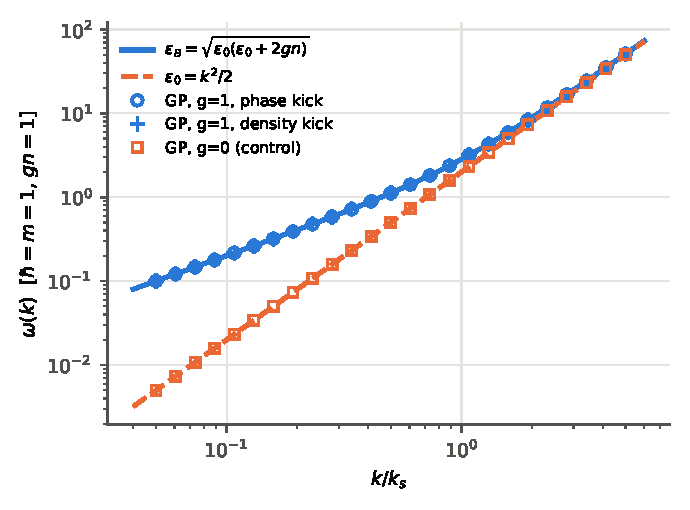
\includegraphics[width=0.49\linewidth]{data/fig_dispersion.pdf}\hfill
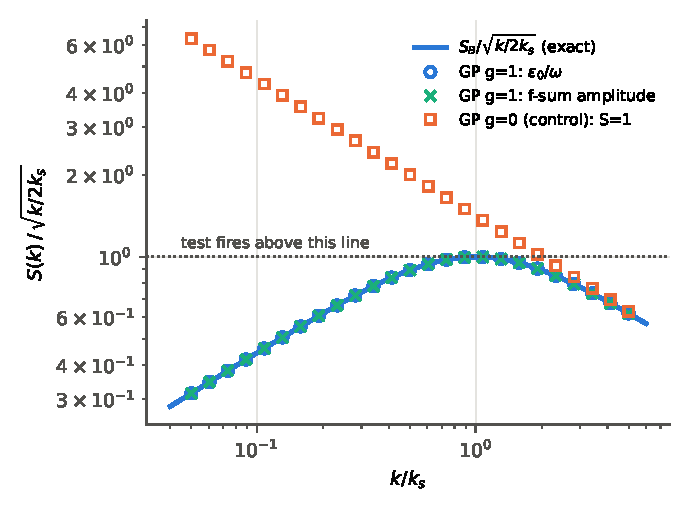
\includegraphics[width=0.49\linewidth]{data/fig_s_over_bound.pdf}
\caption{Left: $\omega(k)$ from GP linear response (phase and density kicks at $g=1$, and the $g=0$ control)
against $\eB$ and $\varepsilon_0$. Right: $S/\sqrt{k/2\ks}$ for the exact $\SB$, the measured $\varepsilon_0/\omega$,
the f-sum amplitude and the $g=0$ control, which exceeds 1 for $k<2\ks$. Generated by \texttt{make\_figures.py} from the
result files. \tier{X}}
\label{fig:disp}
\end{figure}
\begin{figure}[!htb]\centering
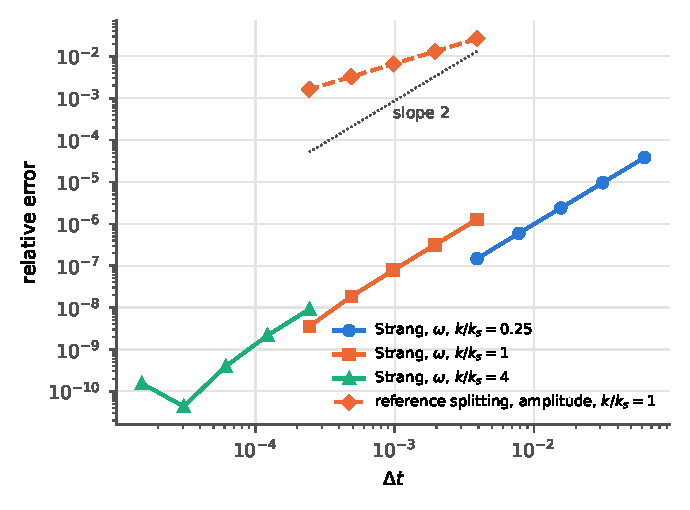
\includegraphics[width=0.5\linewidth]{data/fig_convergence.pdf}
\caption{Strang second-order frequency convergence at three $k$, and the first-order amplitude error of the reference
splitting. \tier{X}}
\label{fig:conv}
\end{figure}

\section{Real-data illustration: superfluid $^4$He}\label{sec:helium}
\paragraph{Inputs \tier{L}.} The dispersion is Godfrin et al.~\cite{godfrin}, Table~VI: $\varepsilon(k)$ at saturated
vapour pressure and $T<100$\,mK, for $k=0$ to $3.6$\,\AA$^{-1}$ in steps of $0.05$ (73 rows). Below $0.15$\,\AA$^{-1}$
the entries are ultrasound data \tier{L, BS-L-0002}. The sound speed is $c=238.3\pm0.1$\,m/s and the molar mass is
$4.0026032$\,g/mol, from the same paper \tier{L, BS-L-0001}. The roton cross-check is Beauvois et al.~\cite{beauvois},
Table~I: $\Delta_R=0.7416(10)$\,meV at $Q_R=1.9260(2)$\,\AA$^{-1}$ \tier{L, BS-L-0003}. The table was transcribed from
the alphaXiv text extraction. The transcription controls pass: uniform $k$ spacing, a table minimum at
$(1.90,\,0.7427)$ against the reference roton, and $\varepsilon(0.05)$ within $\HePhonRel$\% of $\hbar ck$.

\paragraph{Evaluation \tier{X, BS-X-0005}.} The scales are $\ks=2m_4c/\hbar=\HeKs$\,\AA$^{-1}$ and
$\hbar^2/2m_4=\HeHbarTwoM$\,meV\,\AA$^2$. The threshold at the roton is $\sqrt{Q_R/2\ks}=\HeThrQR$, moving to
$\HeThrLo$--$\HeThrHi$ across the $\pm0.1$\,m/s uncertainty in $c$.

A dispersion table cannot measure $S$. Under Feynman's inequality (Step~10) it gives only an upper bound
$S(k)\le S_\mathrm{up}(k)=\varepsilon_0(k)/\varepsilon(k)$, computed conservatively from $\varepsilon-\mathrm{err}$
where Table~VI gives an error bar. At $k=\HeNoErrK$\,\AA$^{-1}$ (ultrasound rows) it gives none, so there
$S_\mathrm{up}$ uses $\varepsilon$ itself and is not conservative; the margins are large ($S_\mathrm{up}$ vs threshold:
\HeNoErrMargins).
For the \HeNSilent{} tabulated points $0.05\le k\le\HeSilentHi$\,\AA$^{-1}$, the computed $S_\mathrm{up}$ lies below
$\sqrt{k/2\ks}$. So, \emph{if} Feynman's inequality holds with the measured branch as the lowest density-channel energy,
the test cannot fire on $^4$He there. A stricter variant takes $\min(\varepsilon-\mathrm{err},\hbar ck)$, allowing for
multi-phonon states near $\hbar ck$ where the dispersion is anomalous. It leaves this set unchanged; at
$k=0.5$\,\AA$^{-1}$, $S_\mathrm{up}=\HeMarginS$ against a threshold of $\HeMarginT$.

For the \HeNUnd{} points from $\HeFirstUnd$\,\AA$^{-1}$ upward the table cannot decide. At the tabulated point nearest
the roton, $k=\HeRotonK$\,\AA$^{-1}$, $S_\mathrm{up}=\HeSupRoton$ is far above the threshold there,
$\sqrt{k/2\ks}=\HeThrRotonTab$ (the threshold at $Q_R=1.9260$\,\AA$^{-1}$ itself is $\HeThrQR$), and only a measured, absolutely normalized $S(k)$ could
decide. Because $S_\mathrm{up}$ is only an upper bound, a dispersion table can never make the test fire. \textbf{We
therefore do not claim that the $^4$He roton peak exceeds $\HeThrQR$.} We found no verified, absolutely normalized $S(Q)$
table. The cold-atom literature does not help for an absolute test: Shammass et al.~\cite{shammass} multiply their
measured $S(k)$ by 1.5 ``in order to agree with the 2D GPE simulation'' \tier{L, BS-L-0004}. Their short-Bragg-pulse
standing-wave method is the experimental analogue of our phase kick.

\paragraph{Dispersion-level comparison \tier{X, BS-X-0006}.} This needs no $S$. With the same $c$, the measured
$\varepsilon/\eB$ is $\HeEpsRatio$ at $k=1.95$\,\AA$^{-1}$, with a minimum of $\HeEpsRatioMin$ at $3.6$\,\AA$^{-1}$.
This is the standard fact that $^4$He is not a weakly interacting gas, read directly from the pinned table.
On the same code path, the Bogoliubov $\SB$ built with the $^4$He $c$ never fires, and $S=1$ fires at every tabulated
$k<2\ks$.

\begin{figure}[!htb]\centering
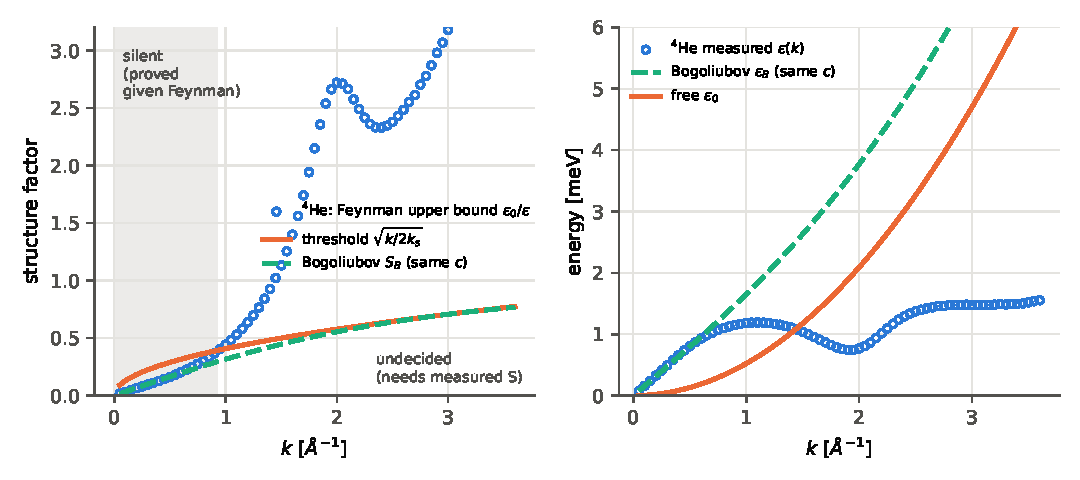
\includegraphics[width=0.62\linewidth]{data/fig_helium.pdf}
\caption{$^4$He from Godfrin et al.\ Table~VI. The Feynman upper bound $\varepsilon_0/\varepsilon$ is plotted against the
threshold $\sqrt{k/2\ks}$, with the silent region shaded, alongside the Bogoliubov $\SB$, and measured $\varepsilon$
against $\eB$ and $\varepsilon_0$. Data \tier{L}, evaluation \tier{X}.}
\label{fig:he}
\end{figure}

\section{HuggingFace dataset search: a null result}\label{sec:hf}
The task asked for a HuggingFace dataset to illustrate the result. We report the search as a null result rather than
substitute an unrelated dataset \tier{X, BS-X-0008}.
\begin{itemize}
\item \textbf{Search.} \HFQueries{} queries were run through \texttt{HfApi.list\_datasets} (public metadata, no token).
They included structure factor (static and dynamic), liquid and superfluid helium, neutron and X-ray diffraction,
Bose--Einstein condensate, Bragg spectroscopy, cold atoms, Bogoliubov, pair and radial distribution function, phonon
and SANS. The full record is \path{data/hf_search.json}.
\item \textbf{Hits.} None of the hits is a measured $S(k)$, $S(Q,\omega)$, Bragg-spectroscopy or cold-atom dataset.
The ``helium'' and ``BEC'' hits are name collisions (language-model checkpoints and other unrelated repositories).
\item \textbf{The single plausible hit} is \texttt{\HFId} at revision \texttt{\HFSha}, tagged MIT. Its card holds
only the licence header. Its data are Python pickles, the largest \HFBig\,GB, named for discriminative ML on 2D
diffraction maps, and nothing identifies them as a liquid or $^4$He $S(Q)$. Only the card and the file list were
fetched (stored under \path{/home/callensxavier_gmail_com/hf-data/bogoliubov_sk/}). Nothing was downloaded or
unpickled, and nothing was substituted.
\end{itemize}
The real-data illustration is therefore the published $^4$He table of Section~\ref{sec:helium}, which is not hosted on
HuggingFace.

\section{Limitations}\label{sec:limits}
\begin{itemize}
\item \textbf{Novelty.} There is none in mathematics or physics. The envelope is an AM--GM corollary of the owner's
\lean{feynman\_ge\_iff} and \lean{ell\_ge}.
\item \textbf{By construction.} \lean{feynman\_sBog\_exact} and \lean{epsBog\_eq\_epsFree\_div\_sBog} hold because
$\SB$ is \emph{defined} as $\varepsilon_0/\eB$. The GP $S=\varepsilon_0/\omega$ inherits this. Nothing here derives
$\SB$ from a many-body calculation.
\item \textbf{Scope of the model.} The model is $T=0$ Bogoliubov only, with no Beliaev damping and no LHY corrections.
\item \textbf{Conditional application.} The dispersion-level test assumes Feynman's inequality (\tier{C}), and applying
it needs $\ks$ from a measured $c$.
\item \textbf{$^4$He.} The roton case is undecided. No absolutely normalized $S(Q)$ source was verified; Svensson et
al.\ and similar diffraction work were not checked and are not cited. A cold-atom paper consulted at Stage~2 (arXiv
cond-mat/0111438) could not be retrieved again at the paper stage and is not cited.
\item \textbf{Verification.} Statement adequacy has been reviewed only by AI agents. The paper-stage recompile is a
second kernel run by another agent instance, not a human audit. The ledger gate flags every Tier~A row as unaudited.
\item \textbf{Protocol and upstream.} The round-1 KEEP came from an out-of-protocol infrastructure retry. The
reused-phase composition seen in the pinned reference data has not been reported upstream, and the upstream Python
source was not inspected.
\item \textbf{Numerics.} All numerics are 2D, classical-field and periodic. They are producer-checked only.
\item \textbf{HuggingFace (unmet deliverable).} The requested HuggingFace illustration was not delivered: no Hub dataset
holds a measured structure factor (Section~\ref{sec:hf}). The $^4$He table stands in as the real-data illustration.
\item \textbf{Tier L scope.} Tier L here is verbatim data and quotes, looser than the Elenchus theorem-only L tier.
\end{itemize}

\section{Claim ledger}\label{sec:ledger}
Every tagged claim is a record in \path{ledger/ledger.json}, built by \path{ledger/build_ledger.py}. Each record points
to a content-addressed evidence blob in \path{ledger/evidence/}:
\begin{itemize}
\item Tier~A: verbatim axiom lines with source and transcript hashes;
\item Tier~L: verbatim excerpts with line numbers and the sha256 of the alphaXiv extraction, copied to
\path{ledger/sources/};
\item Tier~C: the argument text;
\item Tier~X: result files with \texttt{claim\_licence: false}.
\end{itemize}
The Elenchus gate \path{tools/ledger.py ledger.json --evidence-dir evidence} was run on the ledger. Its exit code and
findings are recorded verbatim in \path{ledger/gate_output.txt}. The ledger holds 24 claims (8 A, 4 L, 4 C, 8 X).
The gate exits~1 with 0 blocking findings and 8 flags, one \texttt{LEDGER\_UNAUDITED\_TIER\_A} per Tier~A row, because
no person has audited statement adequacy. A first run (\path{ledger/gate_output_run1.txt}) also blocked a tier
inversion: BS-C-0004 rested on the Tier~X row BS-X-0003. We removed that dependency, so the reading stands as an
unsupported argument. Bookkeeping that passes the gate licenses nothing about truth.

\section{Reproducibility}\label{sec:repro}
\begin{itemize}
\item \textbf{Lean.}
\path{python -I results/autoresearch/2026-10-25/H8/contribution/run_lean_rc2.py FILE.lean OUT.json} from the
AutoevolveAI worktree, for the claimed file and the controls file. The runner pins cores 4--7 and sets
\texttt{LEAN\_PATH} as above.
\item \textbf{Rust.} rusty-SUNDIALS branch \texttt{physics/ar-bogoliubov-2026-10-25}, commits
\texttt{e1449988a91d8a38a7deee7f1106cfa3962c5759} (code and results) and
\texttt{fdd6d2d64fbab0dcaad60fa7b7877d96095c2776} (README, strict $^4$He variant, test log) and
\texttt{ae918316a82f7ac7102d53f646eb20c5a2c838a5} (HEAD; module-doc correction only, results unchanged), not pushed at
the time of writing.
\texttt{cargo build --release -p qf-gpe2d --examples}, then run
\texttt{examples/bogoliubov\_dispersion} (wall time 409\,s, as recorded by the producing agent in
\path{results/autoresearch/2026-10-25/H8/contribution/NUMERICS.md}; it is not written to a machine result file); scripts \texttt{summarize.py}, \texttt{crosscheck\_compare.py},
\texttt{which\_strang.py}, \texttt{helium\_tier\_l.py} and \texttt{make\_figures.py} live in
\path{crates/qf-gpe2d/results/bogoliubov_sk/}.
\item \textbf{Paper.} \texttt{python -I gen\_inputs.py} regenerates every number and listing from the result files.
\texttt{python -I ledger/build\_ledger.py} rebuilds the ledger. \texttt{python -I build\_pdf.py} runs pdflatex twice.
\end{itemize}

\begin{thebibliography}{9}
\bibitem{godfrin} H.~Godfrin, K.~Beauvois, A.~Sultan, E.~Krotscheck, J.~Dawidowski, B.~F{\aa}k, J.~Ollivier,
\emph{The dispersion relation of Landau elementary excitations and the thermodynamic properties of superfluid $^4$He},
arXiv:2012.09067v1 (2020).
\bibitem{beauvois} K.~Beauvois, J.~Dawidowski, B.~F{\aa}k, H.~Godfrin, E.~Krotscheck, J.~Ollivier, A.~Sultan,
\emph{Microscopic dynamics of superfluid $^4$He: a comprehensive study by inelastic neutron scattering},
arXiv:1802.08120v3.
\bibitem{shammass} I.~Shammass, S.~Rinott, A.~Berkovitz, R.~Schley, J.~Steinhauer, \emph{The phonon dispersion relation
of a Bose--Einstein condensate}, arXiv:1207.3440.
\bibitem{feynman} R.~P.~Feynman, Phys.\ Rev.\ \textbf{94}, 262 (1954). This is a bibliographic pointer only, taken
from the reference lists of \cite{godfrin,shammass}; the original was not read for this paper.
\bibitem{qf} SocrateAI-Scientific-QuantumFluids, \path{lean_src/DualLength.lean} at commit
\texttt{10f74daf1b39d2ac51a785452329fff0003cfc83} (owner project; unpublished).
\bibitem{uo} X.~Callens, \emph{Planar universal optimality, tiered} (preprint v2), doi:10.5281/zenodo.23293429; and
\emph{The Triangular Lattice and Universal Optimality} (textbook), doi:10.5281/zenodo.23295142. These are earlier
tiered publications of this programme, cited for method only.
\end{thebibliography}
\noindent The tier conventions and ledger format follow earlier tiered publications of this programme~\cite{uo}. The
owner lemmas come from~\cite{qf}.

\end{document}
